\documentclass[10pt]{beamer}
%\documentclass[handout,10pt]{beamer}
\usepackage{my_style}
%%%%%%%%%%%%%%%%%%%%%%%%%%%%%%%%%%%%%%%%%%%%%%%%%%%%%%%%%%%%%%%%%%%%%%%%

\title[Math/CS 375]{Lecture 06 - C}
\subtitle{\S 8.4 Stability}

\begin{document}
% -------------------------------------------------
\begin{frame}
  \titlepage
\end{frame}
% -------------------------------------------------
\begin{frame}{Goals}
We will answer these questions:\\[3mm]
\begin{itemize}
    \item Why are some systems problematic even if they are non-singular? 
    \item What is a condition number and why is it important? 
    \item What is a residue and what does it represent?
    \item How well can trust the solution to a Gaussian elimination code?
\end{itemize}
\end{frame}
%%%%%%%%%%%%%%%%%%%%%%%%%%%%%%%%%%%%%%%%%%%%%%%%%%%%%%%%%%%%%%%%%%%%%%%
\sectionframe{Visualizing Ill-conditioning}
%%%%%%%%%%%%%%%%%%%%%%%%%%%%%%%%%%%%%%%%%%%%%%%%%%%%%%%%%%%%%%%%%%%%%%%
\begin{frame}{Intersecting lines}
\begin{itemize}
    \item Suppose you want the location where 2 lines intersect 
\begin{align*}
    y &= -2x + 6 \\
    y &= \ \ \frac{1}{2} x + 1
\end{align*}
\item We may write the problem in matrix form
\begin{equation*}
    \left[\negthickspace\begin{array}{cr} 2 & 1 \\ -1/2 & 1 \end{array}\negthickspace\right]
    \begin{bmatrix} x_1 \\ x_2 \end{bmatrix}
    =
    \begin{bmatrix} 6 \\ 1 \end{bmatrix}
\end{equation*}
\item The solution is $x=[2\quad 2]' \implies $ they intersect at $(2,2)$

\item Notice that $A=\left[\negthickspace\begin{array}{cr} 2 & 1 \\ -1/2 & 1 \end{array}\negthickspace\right]$ is nonsingular

\item The lines are \textbf{not parallel} so they must intersect at exactly one point

\end{itemize}
\end{frame}
%%%%%%%%%%%%%%%%%%%%%%%%%%%%%%%%%%%%%%%%%%%%%%%%%%%%%%%%%%%%%%%%%%%%%%%%
\begin{frame}{Four Cases}

\begin{enumerate}
    \item The lines \textbf{intersect}
        \begin{equation*}
            \left[\negthickspace\begin{array}{cr} 2 & 1 \\ -1/2 & 1 \end{array}\negthickspace\right]
            \begin{bmatrix} x_1 \\ x_2 \end{bmatrix}
            =
            \begin{bmatrix} 6 \\ 1 \end{bmatrix}
        \end{equation*}
    \item The lines are \textbf{parallel} and \textbf{distinct} 
    \begin{equation*}
        \begin{bmatrix} 2 & 1 \\ 2 & 1 \end{bmatrix}
        \begin{bmatrix} x_1 \\ x_2 \end{bmatrix}
        =
        \begin{bmatrix} 6 \\ 5 \end{bmatrix}
    \end{equation*}
    % Matrix is singular ($\rank{A}=1$), and the system is inconsistent\\[5pt]


\item The lines are \textbf{parallel} and \textbf{coincident} 
\begin{equation*}
    \begin{bmatrix} 2 & 1 \\ 2 & 1 \end{bmatrix}
    \begin{bmatrix} x_1 \\ x_2 \end{bmatrix}
    =
    \begin{bmatrix} 6 \\ 6 \end{bmatrix}
\end{equation*}

\item The lines are \textbf{nearly parallel}
\begin{equation*}
    \begin{bmatrix} 2 & 1 \\ 2+\delta & 1 \end{bmatrix}
    \begin{bmatrix} x_1 \\ x_2 \end{bmatrix}
    =
    \begin{bmatrix} 6 \\ 6 \end{bmatrix}
\end{equation*}
\end{enumerate}

\end{frame}

%%%%%%%%%%%%%%%%%%%%%%%%%%%%%%%%%%%%%%%%%%%%%%%%%%%%%%%%%%%%%%%%%%%%%%%%
\begin{frame}{Visualizing the Four Cases }

\begin{center}
    \pgfimage[height=6cm]{./figs/systemTypes}

    The nearly parallel case is \textit{very} problematic to handle on the computer.
\end{center}
\end{frame}
%%%%%%%%%%%%%%%%%%%%%%%%%%%%%%%%%%%%%%%%%%%%%%%%%%%%%%%%%%%%%%%%%%%%%%%%

\begin{frame}{Nearly Parallel Case}
\begin{itemize}
    \item Consider \textbf{nearly parallel} case 
    \begin{equation*}
    \begin{bmatrix} 2 & 1 \\ 2+\delta & 1 \end{bmatrix}
    \begin{bmatrix} x_1 \\ x_2 \end{bmatrix}
    =
    \begin{bmatrix} 6 \\ 6\end{bmatrix}
    \end{equation*}
    

    \item In theory, it should have \underline{one unique solution}\\[3mm]

    \item In practice, we may get very inaccurate numerical answers

\end{itemize}
    \question{
    \begin{itemize}
        \item Are there larger $n\times n$ matrices with the same issue? \onslide<2>{\textbf{yes}}
        \item Is there a way to tell if a matrix $A$ has severe issues? \onslide<2>{\textbf{yes}}
        \item Can we quantify the severity of the issue? \onslide<2>{\textbf{yes}}
    \end{itemize}
    }
\end{frame}

%%%%%%%%%%%%%%%%%%%%%%%%%%%%%%%%%%%%%%%%%%%%%%%%%%%%%%%%%%%%%%%%%%%%%%%%
\sectionframe{Linear Algebra Review}
%%%%%%%%%%%%%%%%%%%%%%%%%%%%%%%%%%%%%%%%%%%%%%%%%%%%%%%%%%%%%%%%%%%%%%%%
\begin{frame}[shrink]{Norms}

{\define{Norm}{ The \textbf{norm} of a vector of matrix is a non-negative quantity that represents its size or magnitude. We denote it with $\| \cdot \|$. }}

\begin{block}{Norms of Vectors}
\begin{align*}
    \|x\|_{1} &= |x_1| + |x_2| + \ldots + |x_n| = \sum_{i=1}^{n}{|x_i|}\\
    \|x\|_{\infty} &= \max \left(|x_1|, |x_2|, \ldots, |x_n| \right)
                      = \underset{i}{\max} \left( |x_i| \right)
\end{align*}
\end{block}

\begin{block}{Norms of Matrices}
    
\begin{align*}
  \|A\| &= \max_{x\ne 0} \frac{\|Ax\|}{\|x\|} & \text{theoretical norm}\\
  \|A\|_1 &= \max_{1\leq j \leq n} \sum_{i=1}^{m}|a_{ij}| &\text{largest column sum}\\
  \|A\|_{\infty} &= \max_{1\leq i \leq m} \sum_{j=1}^{n}|a_{ij}| &\text{largest row sum}
\end{align*}
\end{block}
\end{frame}
%%%%%%%%%%%%%%%%%%%%%%%%%%%%%%%%%%%%%%%%%%%%%%%%%%%%%%%%%%%%%%%%%%%%%%%%
\begin{frame}{$p$-Norms}
\begin{itemize}
    \item Vectors:
\begin{align*}
    \|x\|_{p} &= \bigl( |x_1|^p + |x_2|^p + \ldots + |x_n|^p \bigr)^{1/p}
\end{align*}
\item Matrices:
\begin{align*}
  \|A\|_p = \max_{x\ne 0} \frac{\|Ax\|_p}{\|x\|_p}
\end{align*}
    \item $p$ is a real number $p\ge 1$\\[3mm]

    \begin{block}{Euclidean Norm}
    $p=2$ is a special case: 
    $$
    \|x\|_{2} = \sqrt{ |x_1|^2 + |x_2|^2 + \ldots + |x_n|^2 }
    $$
    This is also called the \textbf{Euclidean norm}. This is default norm when you do \texttt{norm(x)} in Matlab. 
    \end{block}
\end{itemize}
\end{frame}
%%%%%%%%%%%%%%%%%%%%%%%%%%%%%%%%%%%%%%%%%%%%%%%%%%%%%%%%%%%%%%%%%%%%%%%%
\begin{frame}
\frametitle{Some Important Properties of Norms}

\begin{block}{Positivity}
$$
     \|x\| \geq 0,\; \textrm{and}\,  \|x\| = 0 \textrm{ only if } x = 0
$$
\end{block}

\begin{block}{Homogeniety}
$$
     \|c x\| = |c| \|x\|
$$
\end{block}

\begin{block}{Submultiplicative (some norms do not have this property)}
$$\|Ax\| \le \|A\| \|x\| $$ 
  $$   \norm{AB} \le \norm{A}\norm{B} $$   
\end{block}

     \begin{block}{Triangle Inequality}
         $$
     \|x+y\| \le \|x\| + \| y \|
         $$
     \end{block}

\begin{center}
    \textit{useful in proofs}
\end{center}
\end{frame}


\begin{frame}{What is an Estimate?}

\begin{itemize}
    \define{Estimation}{\textbf{Estimation} of a variable $x$ refers to finding an approximate upper bound.  }
    \begin{example}
         Estimate the quantity $x = 47 \times 99$
    \end{example}
    \item Since $47<50$ and $99< 100$
    \begin{align*}
        x &= 47 \times 99 \\ 
          & < 50 \times 100 \\ 
          & = 5000 \\
    \end{align*}
    \item Our estimate is $x < 5000$
\end{itemize}    
\end{frame}

\begin{frame}{Estimation Error}

\begin{itemize}
    \item We are mainly interested in \underline{estimating the error} 
    \begin{align*}
        e &= |x-5000| \\
          & =| (47)(99) - 5000| \\  
          & = 5000\left| \frac{47}{50} \frac{99}{100} - 1\right| \\  
          & = 5000\left| .94\times .99 - 1\right| \\
          & \le 5000  \left| .9 - 1\right| = 500\\  
    \end{align*}
    \item Guaranteed my estimate is within 500 of the real solution (4653)
\end{itemize}    
\end{frame}

%%%%%%%%%%%%%%%%%%%%%%%%%%%%%%%%%%%%%%%%%%%%%%%%%%%%%%%%%%%%%%%%%%%%%%
\sectionframe{Perturbations}
%%%%%%%%%%%%%%%%%%%%%%%%%%%%%%%%%%%%%%%%%%%%%%%%%%%%%%%%%%%%%%%%%%%%%%

\begin{frame}{Perturbation}
\begin{center}
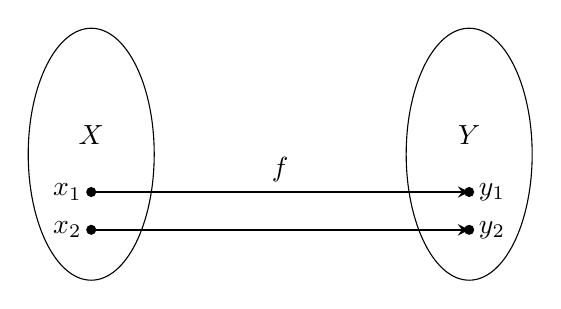
\begin{tikzpicture}[scale=0.8]
% Define sets
% \draw (0,0) circle (1.5cm) node[above] {$X$};
% \draw (6,0) circle (1.5cm) node[above] {$Y$};
\draw (0,0) ellipse (1cm and 2cm) node[above] {$X$};
\draw (6,0) ellipse (1cm and 2cm) node[above] {$Y$};

% Draw elements of sets
\foreach \x in {1,2}{
    \filldraw (0,-\x*0.6) circle (2pt) node[left] {$x_\x$};
    \filldraw (6,-\x*0.6) circle (2pt) node[right] {$y_\x$};
}

% Mapping
\draw[->,>=stealth,thick] (0,-0.6) -- (6,-0.6) node[midway,above] {$f$};
\draw[->,>=stealth,thick] (0,-1.2) -- (6,-1.2);
% \draw[->,>=stealth,thick] (0,-1.8) -- (6,-1.2) node[midway,above] {$f$};
\end{tikzpicture}\\
\textit{small change in input $\implies$ small change in output}
\end{center}

\vspace{4mm}

\begin{itemize}
    \item \textbf{Perturbation} means a small change in a parameter
    \item The mapping $f$ has ``good conditioning" if it is ``stable" with respect to perturbations.
\end{itemize}
\end{frame}

%%%%%%%%%%%%%%%%%%%%%%%%%%%%%%%%%%%%%%%%%%%%%%%%%%%%%%%%%%%%%%%%%%%%%%

\begin{frame}{Perturbation}
\begin{center}
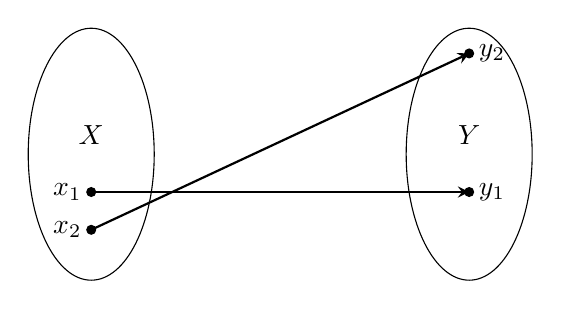
\begin{tikzpicture}[scale=0.8]
% Define sets
% \draw (0,0) circle (1.5cm) node[above] {$X$};
% \draw (6,0) circle (1.5cm) node[above] {$Y$};
\draw (0,0) ellipse (1cm and 2cm) node[above] {$X$};
\draw (6,0) ellipse (1cm and 2cm) node[above] {$Y$};


% Draw elements of sets
\foreach \x in {1,2}{
    \filldraw (0,-\x*0.6) circle (2pt) node[left] {$x_\x$};
    % \filldraw (6,-\x*0.6) circle (2pt) node[right] {$y_\x$};
}

\filldraw (6,-0.6) circle (2pt) node[right] {$y_1$};
\filldraw (6,1.6) circle (2pt) node[right] {$y_2$};

% Mapping
\draw[->,>=stealth,thick] (0,-0.6) -- (6,-0.6);
\draw[->,>=stealth,thick] (0,-1.2) -- (6,1.6);
% \draw[->,>=stealth,thick] (0,-1.8) -- (6,-1.2) node[midway,above] {$f$};
\end{tikzpicture}\\
\textit{small change in input $\implies$ large change in output}
\end{center}

\vspace{4mm}

\begin{itemize}
    \item A mapping $f$ is ``ill-conditioned" if it is ``sensitive" to perturbations.
\end{itemize}
\end{frame}

%%%%%%%%%%%%%%%%%%%%%%%%%%%%%%%%%%%%%%%%%%%%%%%%%%%%%%%%%%%%%%%%%%%%%%
\begin{frame}{Perturbation}
\begin{center}
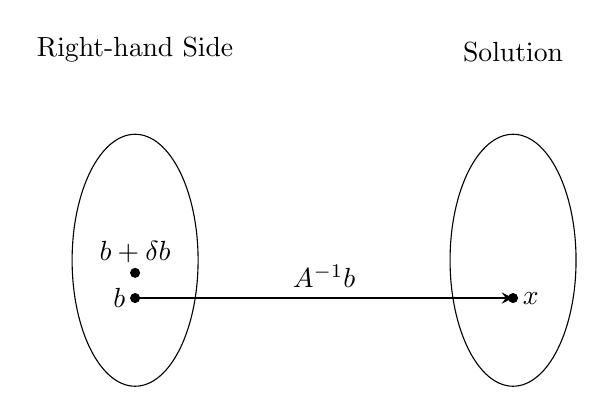
\begin{tikzpicture}[scale=0.8]
% Define sets
% \draw (0,0) circle (1.5cm) node[above] {$X$};
% \draw (6,0) circle (1.5cm) node[above] {$Y$};
\draw (0,0) ellipse (1cm and 2cm); 
\draw (0,3) node[above] {Right-hand Side};
\draw (6,0) ellipse (1cm and 2cm); 
\draw (6,3) node[above] {Solution};


% Draw elements of sets

\filldraw (0,-0.6) circle (2pt) node[left] {$b$};
\filldraw (0,-0.2) circle (2pt) node[above] {$b+\delta b$};
    % \filldraw (6,-\x*0.6) circle (2pt) node[right] {$y_\x$};


\filldraw (6,-0.6) circle (2pt) node[right] {$x$};
% \filldraw (6,1.6) circle (2pt) node[right] {$y_2$};

% Mapping
\draw[->,>=stealth,thick] (0,-0.6) -- (6,-0.6) node[midway,above] {$A^{-1}b$};
% \draw[->,>=stealth,thick] (0,-1.2) -- (6,1.6);
% \draw[->,>=stealth,thick] (0,-1.8) -- (6,-1.2) node[midway,above] {$f$};
\end{tikzpicture}\\
\end{center}

\vspace{4mm}

\begin{itemize}
    \item Suppose we want to solve $Ax=b$.
    \item $b$ gets mapped to $x$
    \item Where does $b+\delta b$ get mapped to?
\end{itemize}
\end{frame}

%%%%%%%%%%%%%%%%%%%%%%%%%%%%%

\begin{frame}{Perturbations to $b$}
\question{
    In the problem $Ax=b$, will a small error $b$ lead to a big change in the solution?
}

\vspace{4mm}

\textbf{Example:}
\begin{itemize}
    \item Suppose the right-hand side of a \matdim{2}{2} system is
\begin{equation*}
    b = \begin{bmatrix}1 \\ 2/3 \end{bmatrix}
\end{equation*}

\item Consider the difference in the two problems
\begin{equation*}
    Ax = \begin{bmatrix}1 \\ 2/3 \end{bmatrix}
    \ \ \ \ \ \ \ \ \
    \text{and}
    \ \ \ \ \ \ \ \ \
    A\hat{x} = \begin{bmatrix}1 \\ 0.6667 \end{bmatrix}
\end{equation*}

\item What can we say about $x$ and $\hat{x}$? 

\end{itemize}
\end{frame}
%%%%%%%%%%%%%%%%%%%%%%%%%%%%%%%%%%%%%%%%%%%%%%%%%%%%%%%%%%%%%%%%%%%%%%
\begin{frame}{Perturbation Notations}
    \begin{itemize}
        \item For our unperturbed problem $Ax=b$, 
            $$x =  \textbf{exact solution}$$
            $$b =  \textbf{exact RHS}$$
        \item We may introduce a small perturbation to the RHS so that $\hat{b} = b + \delta b$ 
            $$\delta b =  \textbf{perturbation to RHS}$$
            $$\hat{b} =  \textbf{perturbed RHS}$$
        \item We may write our perturbed system as $A \hat{x} = \hat{b}$
            $$\hat{x} = x + \delta x_b = \textbf{perturbed solution}$$
            $$\delta x_b = \textbf{perturbation to solution caused by $\delta b$}$$
            
    \end{itemize}
\end{frame}
%%%%%%%%%%%%%%%%%%%%%%%%%%%%%%%%%%%%%%%%%%%%%%%%%%%%%%%%%%%%%%%%%%%%%%
\begin{frame}{Effect of Perturbations to $b$}
\begin{itemize}
    \item Suppose $b$ is perturbed with $\delta b$ such that
        \begin{equation*}
            \frac{\norm{\delta b}}{\norm{b}} \ll 1
        \end{equation*}
    \item Our solution is shifted by $\delta x_b$, i.e. 
        \begin{equation*}
            A (x + \delta x_b) = b + \delta b
        \end{equation*}


    \item Analysis shows (see next two slides for proof) that
        \begin{equation*}
            \frac{\norm{\delta x_b}}{\norm{x}} \le \norm{A}\norm{A^{-1}} \frac{\norm{\delta b}}{{\norm{b}}}
        \end{equation*}

Thus, the effect of the perturbation to $b$ is small
\emph{if} $\norm{A}\norm{A^{-1}}$ is small.
\begin{equation*}
    \text{if }\norm{A}\norm{A^{-1}} \sim 1
    \ \ \ \ \text{then }
    \ \ \ \ \frac{\norm{\delta x_b}}{\norm{x}} \ll 1
\end{equation*}

\end{itemize}
\end{frame}
%%%%%%%%%%%%%%%%%%%%%%%%%%%%%%%%%%%%%%%%%%%%%%%%%%%%%%%%%%%%%%%%%%%%%%%%

\begin{frame}{Proof}{Part 1}
\begin{itemize}
    \item Let $x + \delta x_b$ be the \emph{exact} solution to the perturbed system
\begin{equation}   \label{eq:axdb}
    A (x + \delta x_b) = b + \delta b
\end{equation}
    \item Expand
\begin{equation*}
    Ax + A \delta x_b = b + \delta b
\end{equation*}
    \item Subtract $Ax$ from left side and $b$ from right side since $Ax=b$
\begin{equation*}
    A \delta x_b = \delta b
\end{equation*}
\item Left multiply by $A^{-1}$ to get a formal solution for $\delta x_b$
\begin{equation}   \label{eq:dxb}
    \delta x_b = A^{-1} \delta b
\end{equation}
\end{itemize}
\end{frame}
%%%%%%%%%%%%%%%%%%%%%%%%%%%%%%%%%%%%%%%%%%%%%%%%%%%%%%%%%%%%%%%%%%%%%%%%
\begin{frame}{Proof}{Part 2}
\begin{itemize}
    \item Take norm of equation~\eqref{eq:dxb}
        \begin{equation*}
            \norm{\delta x_b} = \norm{A^{-1}\,\delta b}
        \end{equation*}
    \item Utilize the \textbf{submultiplicative inequality} to get
        \begin{equation}  \label{eq:normdxb}
            \norm{\delta x_b} \le \norm{A^{-1}}\norm{\delta b}
        \end{equation}
    \item Similarly, $Ax=b$ gives $\norm{b} = \norm{Ax}$, and
            \begin{equation}   \label{eq:normb}
                \norm{b} \le \norm{A}\norm{x},
            \end{equation}
    or rather
        \begin{equation}     \label{eq:normxi}
            \frac{1}{\norm{x}} \le \frac{\norm{A}}{\norm{b}}.
        \end{equation}
\end{itemize}
\end{frame}

%%%%%%%%%%%%%%%%%%%%%%%%%%%%%%%%%%%%%%%%%%%%%%%%%%%%%%%%%%%%%%%%%%%%%%%%
\begin{frame}{Proof}{Part 3}

\begin{itemize}
    \item Multiply Equation~\eqref{eq:normxi} by Equation~\eqref{eq:normdxb} to get
        \begin{equation}    \label{eq:dxbonx}
            \frac{\norm{\delta x_b}}{\norm{x}} \le \norm{A}\norm{A^{-1}} \frac{\norm{\delta b}}{{\norm{b}}}   
        \end{equation}

\begin{theorem}
If $x + \delta x_b$ is the \emph{exact} solution to the perturbed system
\begin{equation*}
    A (x + \delta x_b) = b + \delta b
\end{equation*}
then
\begin{equation*}
    \frac{\norm{\delta x_b}}{\norm{x}}
    \le 
    \norm{A}\norm{A^{-1}}
    \frac{\norm{\delta b}}{{\norm{b}}}
\end{equation*}
\end{theorem}

\end{itemize}
\end{frame}
%%%%%%%%%%%%%%%%%%%%%%%%%%%%%%%%%%%%%%%%%%%%%%%%%%%%%%%%%%%%%%%%%%%%%%%%
\begin{frame}{Effect of Perturbations to $b$}

\begin{itemize}
    \item The quantity $\frac{\norm{\delta x_b}}{\norm{x}}$ is the relative error in $x$
        \begin{equation}    \label{eq:dxbonx}
            \frac{\norm{\delta x_b}}{\norm{x}} = \frac{\norm{x - \hat{x} }}{\norm{x}}= \frac{|\textrm{true - approx}|}{|\textrm{true}|}
        \end{equation}

    \item Similarly, the quantity $ \frac{\norm{\delta b}}{{\norm{b}}}$ is the relative error in $b$


\keyidea{

    This theorem actually gives us an error estimate of the solution in terms of the perturbation!
    \begin{equation*}
        \underbrace{\frac{\norm{\delta x_b}}{\norm{x}}}_{\text{rel. error in x}} 
        \le 
        \underbrace{\norm{A}\norm{A^{-1}}}_{\text{some number}} 
        \underbrace{\frac{\norm{\delta b}}{{\norm{b}}}}_{\text{rel. error in b}}
    \end{equation*}
}

\end{itemize}
\end{frame}


%%%%%%%%%%%%%%%%%%%%%%%%%%%%%%%%%%%%%%%%%%%%%%%%%%%%%%%%%%%%%%%%%%%%%%%%
\sectionframe{Condition Number}
%%%%%%%%%%%%%%%%%%%%%%%%%%%%%%%%%%%%%%%%%%%%%%%%%%%%%%%%%%%%%%%%%%%%%%%%
\begin{frame}{Effect of Perturbations to $A$}

{\question{
What if there is error in $A$ with $\delta A$ such that
\begin{equation*}
    \frac{\norm{\delta A}}{\norm{A}} \ll 1 ?
\end{equation*}
}}


\begin{theorem}
For the perturbed system
\begin{equation*}
    (A + \delta A) (x + \delta x_A) = b, 
\end{equation*}
we have
\begin{equation*}
    \frac{\norm{\delta x_A}}{\norm{x + \delta x_A}} \le \norm{A}\norm{A^{-1}} \frac{\norm{\delta A}}{\norm{A}}.
\end{equation*}
\end{theorem}

Thus, the effect of the perturbation to $A$ is small
\emph{if} $\norm{A}\norm{A^{-1}}$ is small.
\begin{equation*}
	\text{if}    \norm{A}\norm{A^{-1}} \sim 1
    \quad \text{then} 
    \quad \frac{\norm{\delta x_A}}{\norm{x + \delta x_A}} \ll 1
\end{equation*}
\end{frame}

%%%%%%%%%%%%%%%%%%%%%%%%%%%%%%%%%%%%%%%%%%%%%%%%%%%%%%%%%%%%%%%%%%%%%%%%
\begin{frame}{Effect of Perturbations to both $A$ and $b$}

{\question{
What if there is error in both $A$ with $\delta A$ and $b$ with $\delta b$ such that
\begin{equation*}
    \frac{\norm{\delta A}}{\norm{A}} \ll 1
    \quad\text{and}\quad
    \frac{\norm{\delta b}}{\norm{b}} \ll 1 ? 
\end{equation*}
}}

\begin{theorem}
For the perturbed system 
\begin{equation*}
    (A + \delta A) (x + \delta x) = b + \delta b, 
\end{equation*}
we have the estimation on the relative error 
\begin{equation*}
    \frac{\norm{\delta x}}{\norm{x}}
    \ \ \le \ \ \norm{A}\norm{A^{-1}} \left[ \frac{\norm{\delta A}}{\norm{A}} + \frac{\norm{\delta b}}{\norm{b}}\right].
\end{equation*}
\end{theorem}
Thus, the effect of the perturbation is small
\emph{if} $\norm{A}\norm{A^{-1}}$ is small.
\begin{equation*}
    \textrm{if } \quad \norm{A}\norm{A^{-1}} \sim 1
    \quad \text{then} \quad
    \frac{\norm{\delta x}}{\norm{x}} \ll 1
\end{equation*}
\end{frame}
%%%%%%%%%%%%%%%%%%%%%%%%%%%%%%%%%%%%%%%%%%%%%%%%%%%%%%%%%%%%%%%%%%%%%%%%
\begin{frame}{Common Factor}

All three theorems have something in common:\\[4mm]
\begin{enumerate}
\item Perturbation in $b$
\begin{equation*}
\frac{\norm{\delta x_b}}{\norm{x}}
\le 
\norm{A}\norm{A^{-1}}
\frac{\norm{\delta b}}{{\norm{b}}}
\end{equation*}

\item Perturbation in $A$
\begin{equation*}
    \frac{\norm{\delta x_A}}{\norm{x + \delta x_A}} \le \norm{A}\norm{A^{-1}} \frac{\norm{\delta A}}{\norm{A}}
\end{equation*}

\item Perturbation in $A$ and $b$
\begin{equation*}
    \frac{\norm{\delta x}}{\norm{x}}
    \ \ \le \ \ \norm{A}\norm{A^{-1}} \left[ \frac{\norm{\delta A}}{\norm{A}} + \frac{\norm{\delta b}}{\norm{b}}\right]
\end{equation*}
\end{enumerate}
\vspace{4mm}
\begin{center}
\onslide<2>{
    They all have the factor $\norm{A}\norm{A^{-1}}$.
}
\end{center}

\end{frame}

%%%%%%%%%%%%%%%%%%%%%%%%%%%%%%%%%%%%%%%%%%%%%%%%%%%%%%%%%%%%%%%%%%%%%%%%
\begin{frame}{Condition number of $A$}
\define{Condition Number}{
The \textbf{condition number} of a square nonsingular matrix is 
\begin{equation*}
    \kappa(A) = \norm{A}\norm{A^{-1}}. 
\end{equation*}
 If $A$ is singular then $\kappa(A) = \infty$. 
}

The condition number is always in the range
\begin{equation*}
    1 \le \kappa(A) \le \infty
\end{equation*}
\begin{quote}
\begin{itemize}
    \item   $\kappa(A)$ is a mathematical property of $A$
    \item   large $\kappa(A) \implies$ $Ax=b$ is sensitive to errors 
    \item   $\kappa(A)$ indicates how close
            $A$ is to being \emph{numerically} singular.
    \item   A matrix with large $\kappa$ is said to be \textbf{ill-conditioned}
    \item Usually computed with 2-norm $\|\cdot\|_2$
\end{itemize}
\end{quote}
\end{frame}
%%%%%%%%%%%%%%%%%%%%%%%%%%%%%%%%%%%%%%%%%%%%%%%%%%%%%%%%%%%%%%%%%%%%%%%%
\begin{frame}{Why is $\kappa\ge 1$?}
\begin{itemize}
    \item In a sense, $\kappa$ numerically describes invertibility of $A$ 
    \item The most easily inverted matrix is the identity $A = I$
    $$
        \kappa(I) = \norm{I}\norm{I^{-1}} =\norm{I}\norm{I} =  1
    $$
    \item You can also prove it explicitly using the submultiplicative inequality 
    \begin{align*}
        \kappa(A) &=  \norm{A}\norm{A^{-1}}\\
                  &\ge  \norm{AA^{-1}}\\
                  &\ge  \norm{I}=  1 \\
    \end{align*}
\end{itemize}
\end{frame}
%%%%%%%%%%%%%%%%%%%%%%%%%%%%%%%%%%%%%%%%%%%%%%%%%%%%%%%%%%%%%%%%%%%%%%%%
\begin{frame}{Significance of $\kappa$}
    \begin{itemize}
        \item The condition number $\kappa(A)$ gives a sense of its severity 

        \item If $\kappa$ was small then this theorem  
        \begin{equation*}
        \frac{\norm{\delta x_b}}{\norm{x}}
        \le 
        \norm{A}\norm{A^{-1}}
        \frac{\norm{\delta b}}{{\norm{b}}}
        \end{equation*}
        says the error in $b$ will \underline{not} cause any issues in the computed answer

        \item If $\kappa$ was large, small errors in $b$ may cause drastic errors in $\delta x_b$ 

        \item In Matlab, use the command \texttt{cond(A)}
    \end{itemize}

    \keyidea{We always expect some mistakes when solving $Ax=b$ due to rounding. The condition number $\kappa$ tells us how much of an impact these small errors will have on the numerical solution.}
\end{frame}


%%%%%%%%%%%%%%%%%%%%%%%%%%%%%%%%%%%%%%%%%%%%%%%%%%%%%%%%%%%%%%%%%%%%%%%%
\sectionframe{Stability}
%%%%%%%%%%%%%%%%%%%%%%%%%%%%%%%%%%%%%%%%%%%%%%%%%%%%%%%%%%%%%%%%%%%%%%%%

\begin{frame}{Stability of an Algorithm}
\begin{center}
\begin{tikzpicture}[
        scale=0.8,
        every node/.style={font=\small},
        >=stealth
    ]
  %--- sets ----------------------------------------------------
  \node[draw, ellipse, minimum width=2cm, minimum height=4cm, align=center] (data)   at (0,0) {Problem\\Data};
  \node[draw, ellipse, minimum width=2cm, minimum height=4cm, align=center] (result) at (6,0) {Result};
  \node[draw, rectangle, minimum width=2.5cm, minimum height=1cm,
        align=center, fill=gray!5] (alg) at (3,-3) {Algorithm to solve $Ax=b$};

  %--- sample inputs / outputs ---------------------------------
  \node (x1) at ($(data.south)+(0, 1.2)$) {$b$};
  \node (x2) at ($(data.south)+(0, 0.8)$) {$\hat{b}$};
  \draw[dashed] (x1) circle (0.8);

  \node (y1) at ($(result.south)+(0, 1.2)$) {$x$};
  \node (y2) at ($(result.north)+(0,-0.5)$) {$\hat{x}$};

  % \foreach \p in {x1,x2,y1,y2}{\fill (\p) circle (2pt);}

  %--- mappings -------------------------------------------------
  \draw[->,thick] (x1) -- (y1) node[midway,above] {$f$};
  \draw[->,thick] (x2) to[out=350,in=190] (y2); % gentle curve

\end{tikzpicture}
\end{center}
\begin{itemize}
    \item \textbf{Stability} is a property of an \textit{algorithm}
    \begin{itemize}
        \item Stable algorithms do not propagate error
    \end{itemize}
    \item Do not confuse it with \textbf{conditioning} which is a property of the problem
\end{itemize}
\end{frame}


%%%%%%%%%%%%%%%%%%%%%%%%%%%%%%%%%%%%%%%%%%%%%%%%%%%%%%%%%%%%%%%%%%%%%%%%
\begin{frame}{A quote from very smart people}
\textbf{In Practice}, applying Gaussian elimination with
partial pivoting and back substitution to $Ax=b$ gives the \textbf{exact
solution}, $\hat{x}$, to the \textbf{nearby problem}
\begin{equation*}
    (A + E)\hat{x} = b
    \ \ \ \
    \text{where}
    \ \ \ \
    \|E\|_{\infty} \le  \epsm \|A\|_{\infty}
\end{equation*}
\begin{quote}
    Gaussian elimination with partial pivoting and back substitution
    ``gives exactly the right answer to nearly the right question.''
    \par\hfill{--- Trefethen and Bau}
\end{quote}

\vspace{4mm}

\onslide<2>{
\begin{block}{The Meaning}
    \begin{itemize}
        \item GE is stable because it limits propagation of rounding error
        \item But GE needs to have partial pivoting
    \end{itemize}
\end{block}
}
\end{frame}
%%%%%%%%%%%%%%%%%%%%%%%%%%%%%%%%%%%%%%%%%%%%%%%%%%%%%%%%%%%%%%%%%%%%%%%%
\begin{frame}{The Residual}

    \question{Suppose we use an algorithm to get $\hat{x}$. In practice, we don't know the true solution to $Ax=b$ so we can't compute error $e = \norm{\hat{x}-x}$. Then how do we know if $\hat{x}$ is accurate?
        }
    \begin{itemize}

    \bigskip

    \define{Residual}{
    
    The \textbf{residual} measures how close $\hat{x}$ is to satisfying
    the original equation
    
    \begin{equation*}
        r = b - A\hat{x}
    \end{equation*}
    We call the magnitude $\norm{r}$ the \textbf{backward error}. 
    }
    \item If $x\approx \hat{x}$, then $Ax\approx A\hat{x}$. Therefore, $A\hat{x}\approx b$ should be small.

    \item The residue gives us a sense of error even if the true solution is not known

    \end{itemize}
\end{frame}
%%%%%%%%%%%%%%%%%%%%%%%%%%%%%%%%%%%%%%%%%%%%%%%%%%%%%%%%%%%%%%%%%%%%%%
\begin{frame}{The Residual Theorem}

{\question{
    How reliable is $\norm{r}$ as a measure of error?
}}

\begin{theorem}
    For a square linear system $Ax=b$, 
\begin{equation*}
    \frac{\norm{\hat{x} - x}}{\norm{\hat{x}}}
       \ \le\ \kappa(A) \frac{\norm{r}}{\norm{A} \, \norm{\hat{x}}}
\end{equation*}
\end{theorem}


\keyidea{Just because the residue is small does not mean your error is small. It depends on the condition number of $A$.}

\end{frame}

%%%%%%%%%%%%%%%%%%%%%%%%%%%%%%%%%%%%%%%%%%%%%%%%%%%%%%%%%%%%%%%%%%%%
\sectionframe{GE Rule of Thumb}
%%%%%%%%%%%%%%%%%%%%%%%%%%%%%%%%%%%%%%%%%%%%%%%%%%%%%%%%%%%%%%%%%%%%

\begin{frame}[fragile]{The Backslash Operator}
\begin{itemize}
    \item The formal solution to a linear problem is given by 
        \begin{equation*}
            Ax = b
            \qquad
            \Longrightarrow
            \qquad
            x = A^{-1}b
        \end{equation*}
        
    \item It is bad practice to do the following 
\begin{lstlisting}[language=matlab]
x = inv(A)*b % solution to A*x = b
\end{lstlisting}

    \vspace{3mm}
    \item Why not?
        \begin{itemize}
            \item \textbf{Accuracy:} $A$ can be ill-conditioned
            \item \textbf{Speed:} Slower than using a specialized solver
            \item \textbf{Memory:} Storing $A^{-1}$ requires an additional $n\times n$ doubles
        \end{itemize}

        \vspace{5mm}
    \item Use this instead - \textbf{backslash operator}
\begin{lstlisting}[language=matlab]
x = A\b % solution to A*x = b
\end{lstlisting}
\end{itemize}

\end{frame}
% ------------
\begin{frame}{What does it do?}

\cols{
\begin{itemize}
\item The backslash operator check's for structure in the $A$ matrix to perform optimal algorithm 
\item Example: if will do back substitution if $A$ is triangular O$(n^2)$ 
\item Last resort: GE with partial pivoting O$(n^3)$ 
\end{itemize}
}{
   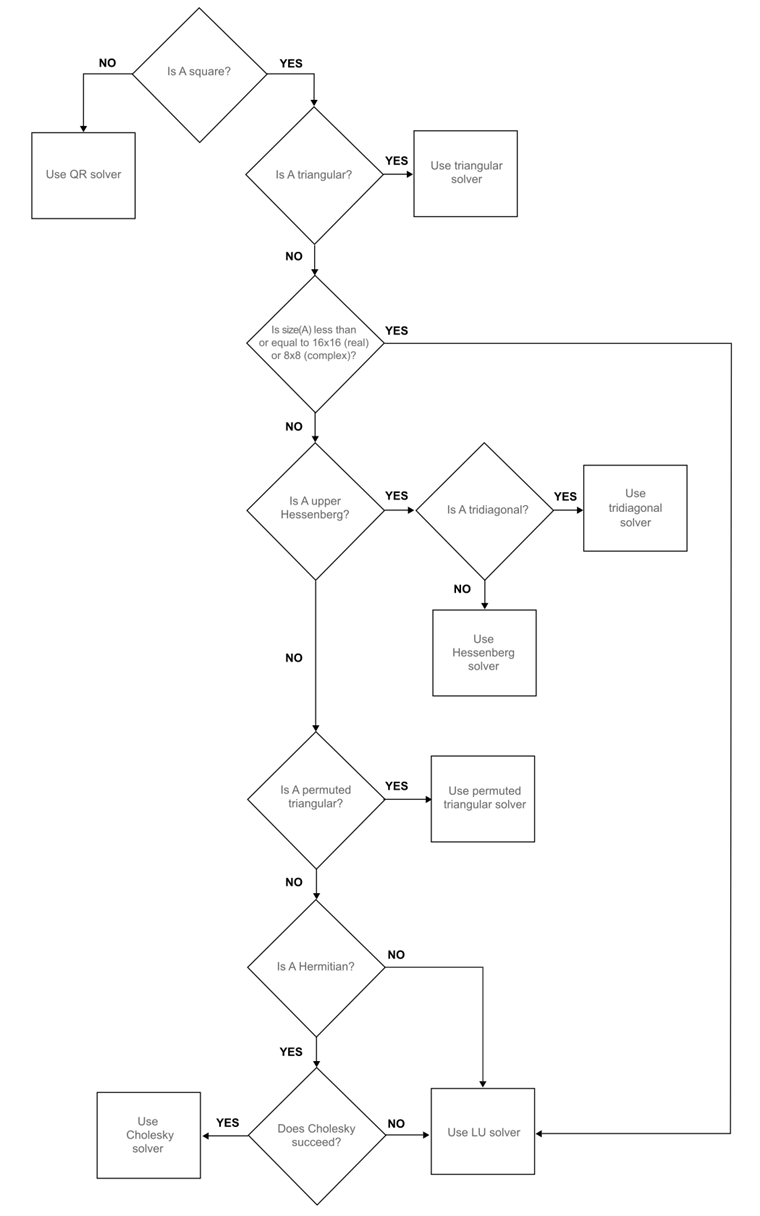
\includegraphics[height=8cm]{figs/mldivide_full.png} 
}
\end{frame}
% --------

\begin{frame}[fragile]{Example Usage}
If you wanted to solve 
$$
\begin{bmatrix}
    1 & 400\\
    3 & 1 
\end{bmatrix} \begin{bmatrix}
    x\\y
\end{bmatrix} = 
\begin{bmatrix}
    3\\4
\end{bmatrix}
$$
in Matlab, you would type
\begin{lstlisting}[language=matlab]
>> A = [1 400; 3 1];
>> b = [3; 4];
>> x = A\b
x =
   1.331943286071726
   0.004170141784821
\end{lstlisting}
\question{Matlab shows the answers up to 15 digits. How many of these digits can we actually trust?}
\end{frame}


% --------
\begin{frame}[fragile]{How many digits can you trust?}

\begin{block}{Rule of Thumb}
If \(A\) and \(b\) are stored to machine precision \(\varepsilon_{\text{m}}\),
then solving \(Ax=b\) with Gaussian elimination with partial pivoting produces a solution
that is accurate to
\[
d \;=\; \bigl|\log_{10}(\varepsilon_{\text{m}})\bigr| - \log_{10}\!\bigl(\kappa(A)\bigr)
\]
significant decimal digits.
\end{block}

\begin{itemize}
  \item The value \(d\) tells you the \underline{number of significant digits} you
        can safely quote.

  \item For example, if in the previous example $d=4$ then 
\begin{Verbatim}[commandchars=\\\{\}]
x =
   1.3319\sout{43286071726}
   0.0041\sout{70141784821}
\end{Verbatim}
All numbers after the 4th place are worthless
\end{itemize}

\end{frame}
%%%%%%%%%%%%%%%%%%%%%%%%%%%%%%%%%%%%%%%%%%%%%%%%%%%%%%%%%%%%%%%%%%%%%%%%
\begin{frame}{Rule of Thumb Example}

\begin{example}
Suppose your system has a condition number $\kappa(A)\sim10^{10}$. If you solve the system using 
FP64 ($\epsm\approx 2.2\times10^{-16}$) then how many correct decimal digits will the solution have?  
\end{example}

We utilize the rule of thumb:
\begin{align*}
	d &= | \log_{10}(\epsm)| - \log_{10}\left(\kappa(A)\right)\\
     &= | \log_{10}(2.2\times10^{-16})| - \log_{10}\left(10^{10}\right) \\
      &\approx 15 - 10  \\
      &= 5 \text{ correct (decimal) digits}
\end{align*}


\onslide<2>{
\keyidea{
    You can initially trust up to 15 or 16 digits in double precision. After performing numerous arithmetic operations to solve for $x$, you lose $\log_{10}(\kappa)$ digits. 
}
}
\end{frame}

% --------------------------

\begin{frame}[fragile]{How many digits can we trust?}

\question{Matlab shows the answers up to 15 digits. How many of these digits can we actually trust?}
\begin{lstlisting}[language=matlab]
>> A = [1 400; 3 1];
>> b = [3; 4];
>> x = A\b
x =
   1.331943286071726
   0.004170141784821

>> d = abs(log10(eps)) - log10(cond(A)) 
d =
  13.528253505318069
\end{lstlisting}
We can trust about 13 digits out of the 15 shown. Effectively our answer is 
\begin{Verbatim}[commandchars=\\\{\}]
x =
   1.3319432860717\sout{26}
   0.0041701417848\sout{21}
\end{Verbatim}
\end{frame}


%%%%%%%%%%%%%%%%%%%%%%%%%%%%%%%%%%%%%%%%%%%%%%%%%%%%%%%%%%%%%%%%%%%%%%%%
\begin{frame}{Summary of Limits to Numerical Solution of $Ax=b$}

\begin{enumerate}
    \item   $\kappa(A)$ indicates how close $A$ is to being numerically singular ($\kappa=1$ being the nicest)\\[5pt]
    \item   If $\kappa(A)$ is ``large'', $A$ is \textbf{ill-conditioned} and
            \emph{even the best} numerical algorithms will produce a solution,
            $\hat{x}$ that cannot be guaranteed to be close to the true
            solution, $x$\\[5pt]
    \item   In practice, Gaussian elimination with partial pivoting and
            back substitution produces a solution with a small residual
            \begin{equation*}
                r = b - A\hat{x}
            \end{equation*}
            \emph{even if} $\kappa(A)$ is large.\\[5pt]
    \item As a rule of thumb you expect to lose $k$ digits of precision where $k=\log_{10}(\kappa)$
\end{enumerate}
\end{frame}

% %%%%%%%%%%%%%%%%%%%%%%%%%%%%%%%%%%%%%%%%%%%%%%%%%%%%%%%%%%%%%%%%%%%%%%%%
% \sectionframe{Matlab's Backslash Operator}
% %%%%%%%%%%%%%%%%%%%%%%%%%%%%%%%%%%%%%%%%%%%%%%%%%%%%%%%%%%%%%%%%%%%%%%%%
% \begin{frame}[fragile]{The Backslash Operator}

% \begin{itemize}
%     \item The formal solution to a linear problem is given by 
%         \begin{equation*}
%             Ax = b
%             \qquad
%             \Longrightarrow
%             \qquad
%             x = A^{-1}b
%         \end{equation*}
        
%     \item It is bad practice to do the following 
% \begin{lstlisting}[language=matlab]
% x = inv(A)*b % solution to A*x = b
% \end{lstlisting}

%     \vspace{3mm}
%     \item Why not?
%         \begin{itemize}
%             \item \textbf{Accuracy:} $A$ can be ill-conditioned
%             \item \textbf{Speed:} Slower than using a specialized solver
%             \item \textbf{Memory:} Storing $A^{-1}$ requires an additional $n\times n$ doubles
%         \end{itemize}

%         \vspace{5mm}
%     \item Use this instead - \textbf{backslash operator}
% \begin{lstlisting}[language=matlab]
% x = A\b % solution to A*x = b
% \end{lstlisting}

% \end{itemize}

% \end{frame}

% %%%%%%%%%%%%%%%%%%%%%%%%%%%%%%%%%%%%%%%%%%%%%%%%%%%%%%%%%%%%%%%%%%%%%%%%
% \begin{frame}[fragile]{The Backslash Operator}

% \question{
%     Why is the backslash operator better?    
% }


% \vspace{0.5cm}
% \begin{enumerate}
%     \item   Does not compute an inverse.
%         \begin{itemize}
%             \item No additional memory requirement
%             \item Avoid unnecessary error propagation
%         \end{itemize}

%     \item   Checks to see if $A$ has a special pattern
%         \begin{itemize}
%             \item Examples: diagonal, tridiagonal, triangular
%             \item Chooses specialized solvers for optimal speed
%         \end{itemize}

%     \item   Defaults to Gaussian elimination with partial pivoting 
%         \begin{itemize}
%             \item At least as good as \texttt{inv(A)}
%         \end{itemize}

%     \item   Has special methods for Sparse and Dense matrices
% \end{enumerate}

% \end{frame}

% %%%%%%%%%%%%%%%%%%%%%%%%%%%%%%%%%%%%%%%%%%%%%%%%%%%%%%%%%%%%%%%%%%%%%%%%
% \begin{frame}{Dense Matrix Flowchart}

% \cols{
% Tries to find the optimal algorithm:
% \begin{itemize}
%     \item Check if $A$ is square 
%     \item Check if $A$ is triangular 
%     \item Check if it's less than $16\times 16$ 
%     \item Check if it's tridiagonal 
%     \item Check if it's symmetric 
%     \item Check if it's symmetric, positive definite 
% \end{itemize}
% }{

%    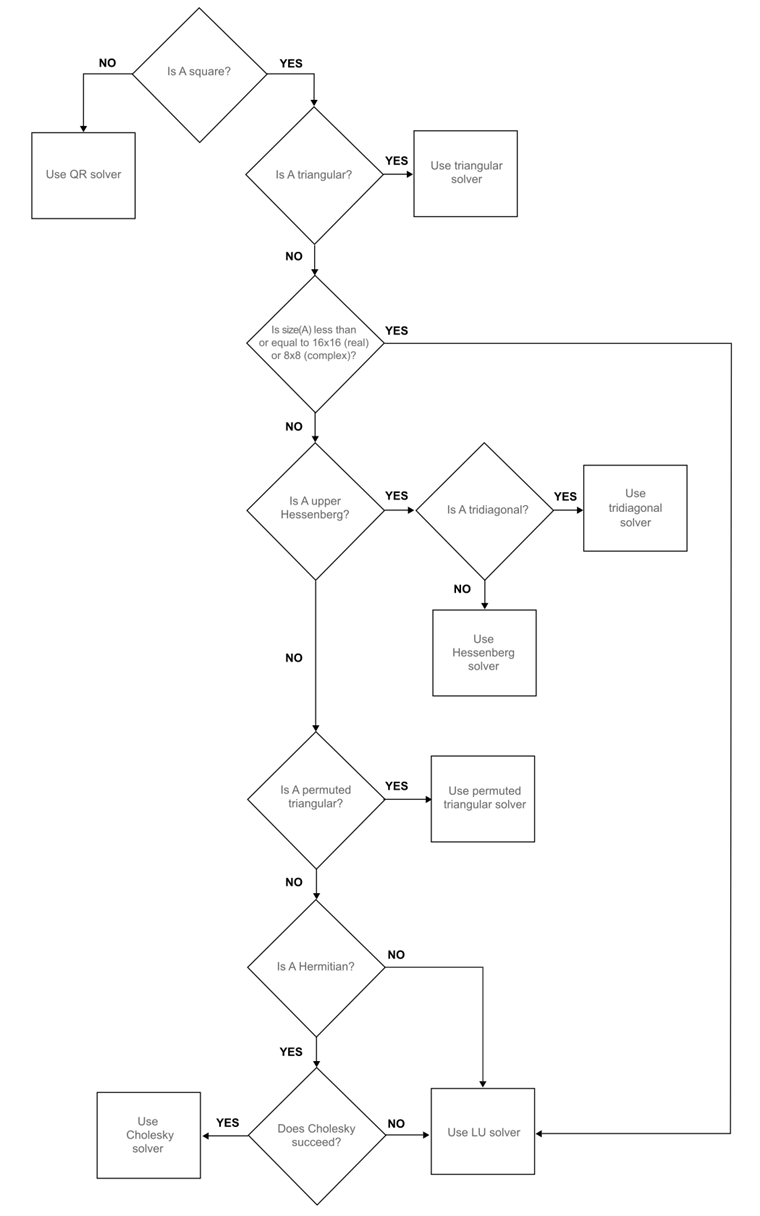
\includegraphics[height=8cm]{figs/mldivide_full.png} 
% }

% \end{frame}


% %%%%%%%%%%%%%%%%%%%%%%%%%%%%%%%%%%%%%%%%%%%%%%%%%%%%%%%%%%%%%%%%%%%%%%%%
% \begin{frame}{Sparse Matrices}
% \define{Sparse and Dense}{A matrix is considered \textbf{sparse} if a large ratio of its elements are zero. A matrix is considered \textbf{dense} if it is not sparse.}

% Examples:
%   \begin{itemize}
%     \item Diagonal 
%     \item Tridiagonal
%     \item Banded 
%     %\item LU decomposition
%     %\item Cholesky factorization
%   \end{itemize}
%   \vspace{3mm}


% Why sparse matrices are important:
% \begin{itemize}
%     \item \textbf{Cheaper memory}: store only non-zero values
%     \item \textbf{Faster routines}: specialized routines skip over zero entries
%     \item \textbf{Applications}: banded matrices frequently arise in solving differential equations
% \end{itemize}


% \end{frame}
% %%%%%%%%%%%%%%%%%%%%%%%%%%%%%%%%%%%%%%%%%%%%%%%%%%%%%%%%%%%%%%%%%%%%%%%%

% \begin{frame}[fragile,shrink]{Sparse Matrices in Matlab}
%     \begin{itemize}
%         \item \texttt{A = sparse(A)}\\ 
%             Change the matrix into sparse format 
%         \item \texttt{A = full(A)}\\ 
%             Change the matrix into dense format 
%         \item \texttt{A = gallery(...)}\\
%             Create one of many specialized matrices (usually sparse)

% \begin{lstlisting}[language=matlab]
% A = gallery('clement',4) % create a Clement matrix of size 4 
% A =
%      0     1     0     0
%      3     0     2     0
%      0     2     0     3
%      0     0     1     0

% A = sparse(A)
% A = 
%    (2,1)        3
%    (1,2)        1
%    (3,2)        2
%    (2,3)        2
%    (4,3)        1
%    (3,4)        3
% \end{lstlisting}
        
%     \end{itemize}
% \end{frame}

% %%%%%%%%%%%%%%%%%%%%%%%%%%%%%%%%%%%%%%%%%%%%%%%%%%%%%%%%%%%%%%%%%%%%%%%%
% \begin{frame}{Sparse Matrix Flowchart}

% \cols{
% Backslash has a different flowchart when $A$ is sparse
% \begin{itemize}
%     \item Square?
%     \item Diagonal? 
%     \item Triangular? 
%     \item Banded? 

%     \item Symmetric? 
%     \begin{itemize}
%         \item Yes $\rightarrow$ Use LDL solver 
%     \end{itemize}
%     \item Symmetric positive definite? 
%     \begin{itemize}
%         \item Yes $\rightarrow$ Use Cholesky solver
%         \item No $\rightarrow$ Use LU solver (GE)
%     \end{itemize}
% \end{itemize}
% }{
%    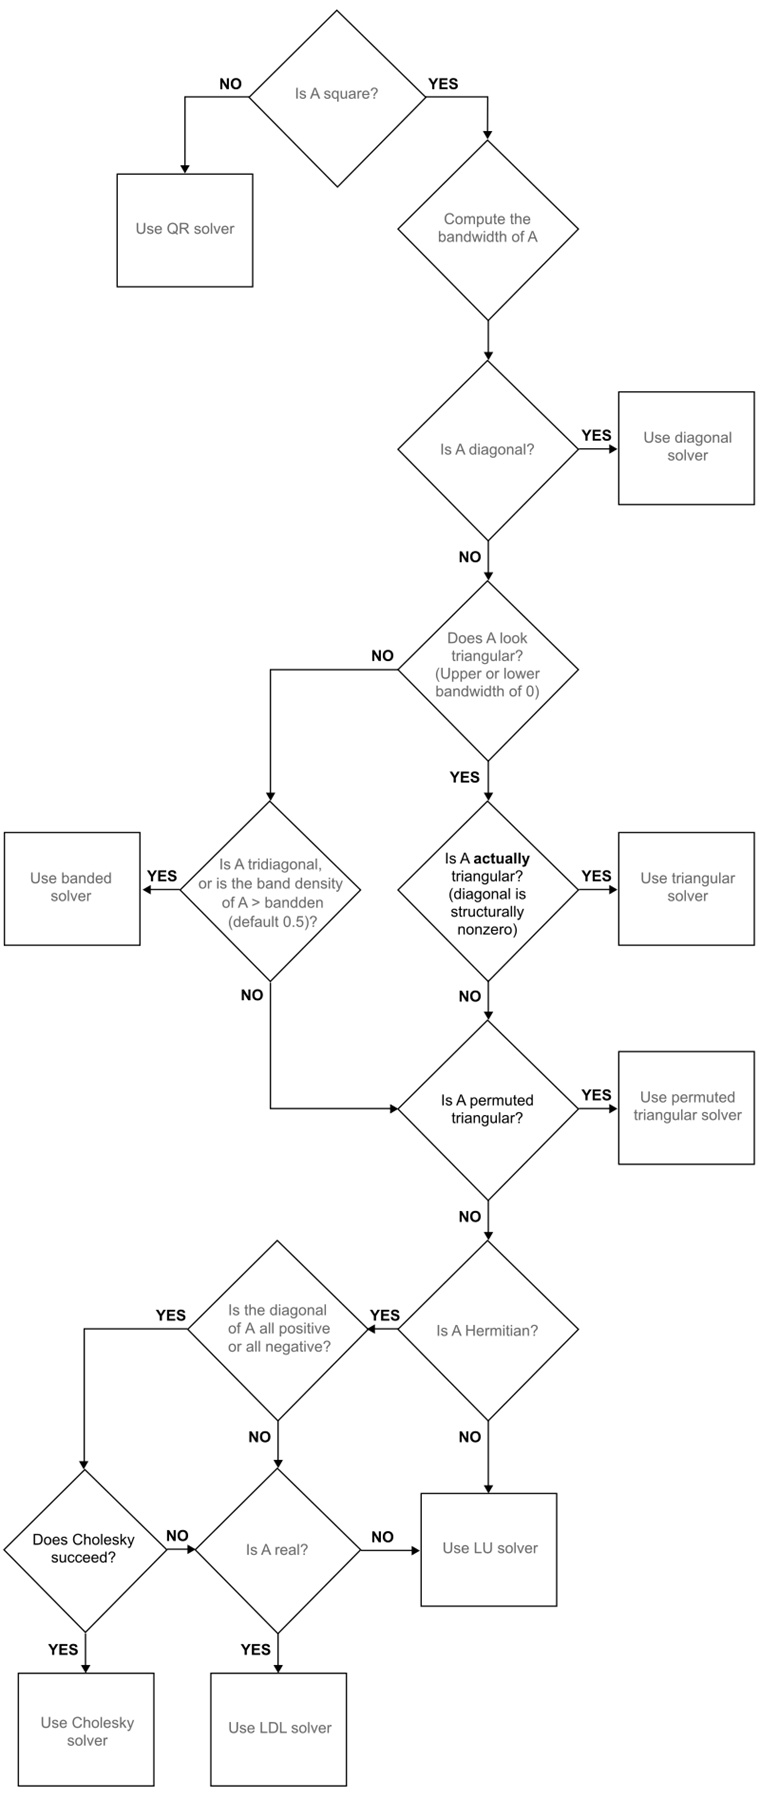
\includegraphics[height=8cm]{figs/mldivide_sparse.png} 
% }

% \end{frame}
% %%%%%%%%%%%%%%%%%%%%%%%%%%%%%%%%%%%%%%%%%%%%%%%%%%%%%%%%%%%%%%%%%%%%%%%%
% \begin{frame}{Moving Forward}

% {\keyidea{
% \begin{itemize}
%     \item GE with partial pivoting is available in Matlab - use the \textbf{backslash operator}
%     \item It will automatically use a better algorithm in special cases
%     \item Use the rule of thumb to determine its significance 
%     \[
%     d \;=\; \bigl|\log_{10}(\varepsilon_{\text{m}})\bigr| - \log_{10}\!\bigl(\kappa(A)\bigr)
%     \]
% \end{itemize}
% }}

% \question{
% \begin{itemize}
%     \item Why is GE listed as ``LU solver"? 
%     \item What is an ``LDL solver"? 
%     \item What is a ``Cholesky solver"? 
% \end{itemize}
% }
% \end{frame}
%%%%%%%%%%%%%%%%%%%%%%%%%%%%%%%%%%%%%%%%%%%%%%%%%%%%%%%%%%%%%%%%%%%%%%%%
\end{document}
